\setcounter{subsection}{2-1}
\subsection{Functions}

% Some useful macros for this section
\def\ivf{\inv{f}}
\def\ivg{\inv{g}}

\exercise{1}{
  Let $f: A \to B$.
  Let $A_0 \ss A$ and $B_0 \ss B$.
  \eparts{
  \item Show that $A_0 \ss \ivf(f(A_0))$ and that equality holds if $f$ is injective.
  \item Show that $f(\ivf(B_0)) \ss B_0$ and that equality holds if $f$ is surjective.
  }
}
\sol{
  \dwhitman

  (a)
  \qproof{
    Consider any $x \in A_0$ and let $y = f(x)$ so that clearly $y \in f(A_0)$.
    Then, since $f(x) = y \in f(A_0)$, it follows from the definition of the preimage that $x \in \ivf(f(A_0))$.
    Hence $A_0 \ss \ivf(f(A_0))$ as desired since $x$ was arbitrary.
    Now suppose that $f$ is also injective and consider this time any $x \in \ivf(f(A_0))$ so that $y = f(x) \in f(A_0)$ by the definition of a preimage.
    Then there is an $x' \in A_0$ where $f(x') = y = f(x)$ by the definition of an image.
    Since $f$ injective though, it must be that $x = x' \in A_0$.
    This shows that $\ivf(f(A_0)) \ss A_0$ since $x$ was arbitrary.
    The desired equality follows since it was already shown that $A_0 \ss \ivf(f(A_0))$ (whether or not $f$ is injective). 
  }

  (b)
  \qproof{
    First suppose that $y$ is any element of $f(\ivf(B_0))$ so that there is an $x \in \ivf(B_0)$ where $f(x) = y$.
    Since $x \in \ivf(B_0)$, we then have that $y = f(x) \in B_0$ by the definition of a preimage.
    Hence $f(\ivf(B_0)) \ss B_0$ since $y$ was arbitrary.
    Now suppose also that $f$ is surjective and suppose that $y \in B_0$ so that also clearly $y \in B$ since $B_0 \ss B$.
    Since $f$ is surjective, there is an $x \in A$ where $f(x) = y$.
    We then have that $x \in \ivf(B_0)$ since $f(x) = y \in B_0$.
    Clearly then $y = f(x) \in f(\ivf(B_0))$ so that $B_0 \ss f(\ivf(B_0))$ since $y$ was arbitrary.
    This shows equality as desired.
  }
}

\exercise{2}{
  Let $f: A \to B$ and let $A_i \ss A$ and $B_i \ss B$ for $i=0$ and $i=1$.
  Show that $\ivf$ preserves inclusions, unions, intersections, and differences of sets:
  \eparts{
  \item $B_0 \ss B_1 \imp \ivf(B_0) \ss \ivf(B_1)$.
  \item $\ivf(B_0 \cup B_1) = \ivf(B_0) \cup \ivf(B_1)$.
  \item $\ivf(B_0 \cap B_1) = \ivf(B_0) \cap \ivf(B_1)$.
  \item $\ivf(B_0 - B_1) = \ivf(B_0) - \ivf(B_1)$.
  }
  Show that $f$ preserves inclusions and unions only:
  \eparts[4]{
  \item $A_0 \ss A_1 \imp f(A_0) \ss f(A_1)$.
  \item $f(A_0 \cup A_1) = f(A_0) \cup f(A_1)$.
  \item $f(A_0 \cap A_1) \ss f(A_0) \cap f(A_1)$; show that equality holds if $f$ injective.
  \item $f(A_0 - A_1) \sps f(A_0) - f(A_1)$; show that equality holds if $f$ injective.
  }
}
\sol{
  \dwhitman

  (a)
  \qproof{
    Suppose that $B_0 \ss B_1$ and consider any $x \in \ivf(B_0)$.
    Then by the definition of a preimage, we have $f(x) \in B_0$ so that also $f(x) \in B_1$ since $B_0 \ss B_1$.
    This shows that $x \in \ivf(B_1)$ again by the definition of a preimage.
    Thus $\ivf(B_0) \ss \ivf(B_1)$ since $x$ was arbitrary as desired.
  }


  (b)
  \qproof{
    We can show this easily using a string of biconditionals.
    For any $x \in A$ we have
    \ali{
      x \in \ivf(B_0 \cup B_1) &\bic f(x) \in B_0 \cup B_1 \\
      &\bic f(x) \in B_0 \lor f(x) \in B_1 \\
      &\bic x \in \ivf(B_0) \lor x \in \ivf(B_1) \\
      &\bic x \in \ivf(B_0) \cup \ivf(B_1) \,,
    }
    which shows the desired result.
  }

  (c)
  \qproof{
    We can show this in a very similar manner to what was done in part (b).
    We have
    \ali{
      x \in \ivf(B_0 \cap B_1) &\bic f(x) \in B_0 \cap B_1 \\
      &\bic f(x) \in B_0 \land f(x) \in B_1 \\
      &\bic x \in \ivf(B_0) \land x \in \ivf(B_1) \\
      &\bic x \in \ivf(B_0) \cap \ivf(B_1) \,,
    }
    for any $x \in A$.
  }

  (d)
  \qproof{
    This is also shown similarly.
    For $x \in A$ we have
    \ali{
      x \in \ivf(B_0 - B_1) &\bic f(x) \in B_0 - B_1 \\
      &\bic f(x) \in B_0 \land f(x) \notin B_1 \\
      &\bic x \in \ivf(B_0) \land x \notin \ivf(B_1) \\
      &\bic x \in \ivf(B_0) - \ivf(B_1) \,.
    }
  }

  (e)
  \qproof{
    Suppose that $A_0 \ss A_1$ and consider any $y \in f(A_0)$.
    Then there is an $x \in A_0$ where $y = f(x)$ by the definition of an image set.
    Then also $x \in A_1$ since $A_0 \ss A_1$, from which it follows that $y = f(x) \in f(A_1)$.
    Therefore $f(A_0) \ss f(A_1)$ as desired since $y$ was arbitrary.
  }

  (f)
  \qproof{
    We can show this easily using a string of biconditionals.
    For any $x \in A$ we have
    \ali{
      y \in f(A_0 \cup A_1) &\bic \exists x (x \in A_0 \cup A_1 \land y = f(x)) \\
      &\bic \exists x [(x \in A_0 \lor x \in A_1) \land y = f(x)] \\
      &\bic \exists x [(x \in A_0 \land y = f(x)) \lor (x \in A_1 \land y = f(x))] \\
      &\bic \exists x (x \in A_0 \land y = f(x)) \lor \exists x (x \in A_1 \land y = f(x)) \\
      &\bic y \in f(A_0) \lor y \in f(A_1) \\
      &\bic y \in f(A_0) \cup f(A_1) \,,
    }
    which shows the desired result.
  }

  (g)
  \qproof{
    Consider any $y \in f(A_0 \cap A_1)$ so that there is an $x \in A_0 \cap A_1$ where $y = f(x)$.
    Hence of course $x \in A_0$ and $x \in A_1$.
    Since also $y = f(x)$, this suffices to show that $y \in f(A_0)$ and $y \in f(A_1)$, and therefore $y \in f(A_0) \cap f(A_1)$ as desired.

    Now suppose that $f$ is injective and consider any $y \in f(A_0) \cap f(A_1)$.
    Then $y \in f(A_0)$ and $y \in f(A_1)$, from which it follows that there is an $x_0 \in A_0$ where $y = f(x_0)$, and an $x_1 \in A_1$ where $y = f(x_1)$.
    We then have $f(x_0) = y = f(x_1)$ so that $x_0 = x_1$ since $f$ is injective.
    Hence $x_0 \in A_0$ and $x_0 = x_1 \in A_1$, so of course $x_0 \in A_0 \cap A_1$.
    Since also $y = f(x_0)$, this shows by definition that $y \in f(A_0 \cap A_1)$.
    Therefore $f(A_0) \cap f(A_1) \ss f(A_0 \cap A_1)$ since $y$ was arbitrary, which shows the desired equivalence since the other direction was already shown.
  }

  (h)
  \qproof{
    Consider any $y \in f(A_0) - f(A_1)$ so that $y \in f(A_0)$ and $y \notin f(A_1)$.
    Then there is an $x \in A_0$ where $y = f(x)$.
    We also have that there is no $x' \in A_1$ such that $y = f(x')$.
    Since we know that $y = f(x)$ it then has to be that $x \notin A_1$.
    Hence $x \in A_0 - A_1$, so that $y \in f(A_0 - A_1)$ since of course $y = f(x)$.
    This shows that $f(A_0 - A_1) \sps f(A_0) - f(A_1)$ as desired since $y$ was arbitrary.

    Now suppose that $f$ is injective and consider any $y \in f(A_0 - A_1)$.
    Then there is an $x \in A_0 - A_1$ where $y = f(x)$ by the definition of an image set.
    Then $x \in A_0$ but $x \notin A_1$.
    It then follows that $y \in f(A_0)$ since $y = f(x)$ and $x \in A_0$.
    Consider any $x' \in A_1$.
    Then it cannot be that $y = f(x')$, because if this were the case then $f(x) = y = f(x')$ so that $x = x'$ since $f$ is injective.
    But we know that $x' = x \notin A_1$, which would present a contradiction.
    So it must be that there is no $x' \in A_1$ where $y = f(x')$, which suffices to show that $y \notin f(A_1)$.
    Therefore $y \in f(A_0) - f(A_1)$ so that $f(A_0 - A_1) \ss f(A_0) - f(A_1)$ since $y$ was arbitrary.
    This of course shows equivalence as desired.
  }
}

\exercise{3}{
  Show that (b), (c), (f), and (g) of Exercise~2 hold for arbitrary unions and intersections.
}
\sol{
  \dwhitman

  In what follows suppose that $f: A \to B$ and that $\cA$ and $\cB$ are nonempty collections of subsets of $A$ and $B$, respectively.
  This is to say that $A' \ss A$ for all $A' \in \cA$ and $B' \ss B$ for all $B' \in \cB$.

  First we show that part in Exercise~2.2 part (b) holds for arbitrary unions, i.e. that
  \gath{
    \ivf\parens{\bigcup_{B' \in \cB} B'} = \bigcup_{B' \in \cB} \ivf(B') \,.
  }
  \qproof{
    As before, we again show this with a string of biconditional assertions:
    \ali{
      x \in \ivf\parens{\bigcup_{B' \in \cB} B'} &\bic f(x) \in \bigcup_{B' \in \cB} B' \\
      &\bic \exists B' \in \cB (f(x) \in B') \\
      &\bic \exists B' \in \cB (x \in \ivf(B')) \\
      &\bic x \in \bigcup_{B' \in \cB} \ivf(B')
    }
    as desired.
  }

  Next we show Exercise~2.2 part (c) for arbitrary intersections, that is
  \gath{
    \ivf\parens{\bigcap_{B' \in \cB} B'} = \bigcap_{B' \in \cB} \ivf(B') \,.
  }
  \qproof{
    We show this with a string of bijections again:
    \ali{
      x \in \ivf\parens{\bigcap_{B' \in \cB} B'} &\bic f(x) \in \bigcap_{B' \in \cB} B' \\
      &\bic \forall B' \in \cB (f(x) \in B') \\
      &\bic \forall B' \in \cB (x \in \ivf(B')) \\
      &\bic x \in \bigcap_{B' \in \cB} \ivf(B') \,,
    }
    which shows the desired result.
  }

  Now we show Exercise~2.2 part (f) for arbitrary unions, that is that
  \gath{
    f\parens{\bigcup_{A' \in \cA} A'} = \bigcup_{A' \in \cA} f(A') \,.
  }
  \qproof{
    Again we utilize a string of biconditionals:
    \ali{
      y \in f\parens{\bigcup_{A' \in \cA} A'} &\bic \exists x \squares{x \in \bigcup_{A' \in \cA} A' \land y = f(x)} \\
      &\bic \exists x \squares{\exists A' \in \cA (x \in A') \land y = f(x)} \\
      &\bic \exists x \squares{\exists A' \in \cA (x \in A' \land y = f(x))} \\
      &\bic \exists x \exists A' \in \cA (x \in A' \land y = f(x)) \\
      &\bic \exists A' \in \cA \exists x (x \in A' \land y = f(x)) \\
      &\bic \exists A' \in \cA \squares{\exists x (x \in A' \land y = f(x))} \\
      &\bic \exists A' \in \cA \squares{y \in f(A')} \\
      &\bic y \in \bigcup_{A' \in \cA} f(A') \,,
    }
    from which the result follows immediately.
  }

  Lastly, we show Exercise~2.2 part (g) for arbitrary intersections, which is that
  \gath{
    f\parens{\bigcap_{A' \in \cA} A'} \ss \bigcap_{A' \in \cA} f(A') \,,
  }
  where equality holds if $f$ is injective.
  \qproof{
    First suppose that $y \in f\parens{\bigcap_{A' \in \cA} A'}$ so that there is an $x \in \bigcap_{A' \in \cA} A'$ where $y = f(x)$.
    Then $x \in A'$ for every $A' \in \cA$.
    So, for any such $A' \in \cA$, we have that $x \in A'$ and $y = f(x)$ so that $y \in f(A')$.
    Since $A'$ was arbitrary, this shows that $y \in \bigcap_{A' \in \cA} f(A')$, which shows the desired result since $y$ was arbitrary.

    Now suppose that $f$ is injective and let $y \in \bigcap_{A' \in \cA} f(A')$.
    Then $y \in f(A')$ for every $A' \in \cA$.
    So, for any such $A_0 \in \cA$ we have that $y \in f(A_0)$ so that there is a $x_0 \in A_0$ where $y = f(x_0)$.
    Suppose for the moment that $x_0 \notin \bigcap_{A' \in \cA} A'$ so that there is an $A_1 \in \cA$ where $x_0 \notin A_1$.
    However, since $A_1 \in \cA$ we have that $y \in f(A_1)$, and hence there is an $x_1 \in A_1$ where $y = f(x_1)$.
    But then we have $f(x_0) = y = f(x_1)$ so that $x_0 = x_1$ since $f$ is injective, and so we have that both $x_0 \notin A_1$ and $x_0 = x_1 \in A_1$.
    As this is a contradiction, it has to be that $x_0 \in \bigcap_{A' \in \cA} A'$.
    Since also $y = f(x_0)$, this shows that $y \in f\parens{\bigcap_{A' \in \cA} A'}$.
    This shows that $f\parens{\bigcap_{A' \in \cA} A'} \sps \bigcap_{A' \in \cA} f(A')$ since $y$ was arbitrary, which in turns proves the desired equivalence.
  }
}

\exercise{4}{
  Let $f: A \to B$ and $g: B \to C$.
  \eparts{
  \item If $C_0 \ss C$, show that $\inv{(g \circ f)}(C_0) = \ivf(\ivg(C_0))$.
  \item If $f$ and $g$ are injective, show that $g \circ f$ is injective.
  \item If $g \circ f$ is injective, what can you say about the injectivity of $f$ and $g$?
  \item If $f$ and $g$ are surjective, show that $g \circ f$ is surjective.
  \item If $g \circ f$ is surjective, what can you say about the surjectivity of $f$ and $g$?
  \item Summarize your answers to (b)-(e) in the form of a theorem.
  }
}
\sol{
  \dwhitman

  (a)
  \qproof{
    Suppose that $C_0 \ss C$.
    We can show this with a string of biconditionals.
    For any $x$, we have
    \ali{
      x \in \inv{(g \circ f)}(C_0) &\bic (g \circ f)(x) \in C_0 \\
      &\bic g(f(x)) \in C_0 \\
      &\bic f(x) \in \ivg(C_0) \\
      &\bic x \in \ivf(\ivg(C_0)) \,,
    }
    which of course shows the desired result.
  }

  (b)
  \qproof{
    Suppose that $x,y \in A$ and $x \neq y$.
    Then, since $f$ is injective, it has to be that $f(x) \neq f(y)$ by the contrapositive of the definition of an injection.
    Then again $(g \circ f)(x) = g(f(x)) \neq g(f(y)) = (g \circ f)(y)$ since $f(x) \neq f(y)$ and $g$ is injective.
    This shows that $g \circ f$ is injective by the contrapositive of the definition.
  }

  (c)
  Here we claim that if $g \circ f$ is injective, then $f$ must be injective but $g$ may not be.
  \qproof{
    Suppose that $g \circ f$ is injective but that $f$ is not.
    Then there are $x,y \in A$ where $x \neq y$ but $f(x) = f(y)$.
    Then we have
    \gath{
      (g \circ f)(x) = g(f(x)) = g(f(y)) = (g \circ f)(y) \,,
    }
    which contradicts the fact that $g \circ f$ is injective since $x \neq y$.
    So it must be that $f$ is injective.

    To show that $g$ need not be injective, consider the sets
    \ali{
      A &= \braces{1,2} &
      B &= \braces{1,2,3} &
      C &= \braces{a,b}
    }
    and the function sets
    \ali{
      f &= \braces{(1,1), (2,2)} &
      g &= \braces{(1,a), (2,b), (3,b)} \,.
    }
    It is easy to see that $f: A \to B$ is injective as is the composition $g \circ f = \braces{(1,a), (2,b)}$, but that $g: B \to C$ is not since $g(2) = b = g(3)$.
  }

  (d)
  \qproof{
    Suppose that $f$ and $g$ are surjective and consider any $z \in C$.
    Then there is a $y \in B$ where $z = g(y)$ since $g$ is surjective.
    Since $f$ is also surjective, there is then an $x \in A$ where $y = f(x)$.
    Then we have
    \gath{
      (g \circ f)(x) = g(f(x)) = g(y) = z \,,
    }
    which shows that $g \circ f$ is surjective as desired since $z$ was arbitrary.
  }

  (e)
  We claim that if $g \circ f$ is surjective, then $g$ must be surjective, but $f$ may not be.
  \qproof{
    Suppose that $g \circ f$ is surjective and consider any $z \in C$ so that there is an $x \in A$ where $(g \circ f)(x) = z$.
    Then we have that $g(f(x)) = z$ so that $y = f(x)$ is an element of $B$ where $g(y) = z$.
    This shows that $g$ is surjective since $z$ was arbitrary.

    To show that $f$ need not be surjective we can use the same example sets $A,B,C$ and functions $f,g$ used in part (c).
    It is easy to see there that $g \circ f$ and $g$ are surjective but $f$ is not since there is no element of $A$ that maps to $3 \in B$.
  }

  (f) We can summarize these facts in the following theorem, whose proof is of course found in the previous parts:
  \begin{thrm}
    Suppose that $f: A \to B$ and $g: B \to C$.
    We assert the following:
    \lparts{
    \item If $f$ and $g$ are injective then $g \circ f$ is injective.
    \item If $g \circ f$ is injective then $f$ is also injective.
    \item If $f$ and $g$ are surjective then $g \circ f$ is surjective.
    \item If $g \circ f$ is surjective then $g$ is also surjective.
    }
  \end{thrm}
}

\exercise{5}{
  In general, let us denote the \boldit{identity function} for a set $C$ by $i_C$.
  That is, define $i_C: C \to C$ to be the function given by the rule $i_C(x) = x$ for all $x \in C$.
  Given $f: A \to B$, we say that $g: B \to A$ is a \boldit{left inverse} for $f$ if $g \circ f = i_A$; and we say that $h: B \to A$ is a \boldit{right inverse} for $f$ if $f \circ h = i_B$.
  \eparts{
  \item Show that if $f$ has a left inverse, $f$ is injective; and if $f$ has a right inverse, $f$ is surjective.
  \item Give an example of a function that has a left inverse but no right inverse.
  \item Give an example of a function that has a right inverse but no left inverse.
  \item Can a function have more than one left inverse? More than one right inverse?
  \item Show that if $f$ has both a left inverse $g$ and a right inverse $h$, then $f$ is bijective and $g = h = \ivf$.
  }
}
\sol{
  \dwhitman

  In what follows we suppose that $f: A \to B$.
  
  (a)
  \qproof{
    First suppose that $f$ has a left inverse $g: B \to A$ so that $g \circ f = i_A$.
    Consider any $x,y \in A$ where $f(x) = f(y)$.
    Then we have
    \gath{
      x = i_A(x) = (g \circ f)(x) = g(f(x)) = g(f(y)) = (g \circ f)(y) = i_A(y) = y \,,
    }
    which shows that $f$ is injective by definition.

    Now suppose that $f$ has a right inverse $h: B \to A$ so that $f \circ h = i_B$.
    Consider any $y \in B$ so that
    \gath{
      y = i_B(y) = (f \circ h)(y) = f(h(y)) \,.
    }
    Then $x = h(y)$ is an element of $A$ such that $f(x) = y$, which shows that $f$ must be surjective since $y$ was arbitrary.
  }

  (b) Consider the sets
  \ali{
    A &= \braces{1,2} &
    B &= \braces{a,b,c}
  }
  and the function $f = \braces{(1,a), (2,b)}$.
  Define the function $g: B \to A$ by $g = \braces{(a,1), (b,2), (c,2)}$.
  It is easy to see that this is a left inverse of $f$ since we have
  \ali{
    (g \circ f)(1) &= g(f(1)) = g(a) = 1 &
    (g \circ f)(2) &= g(f(2)) = g(b) = 2
  }
  so that $g \circ f = i_A$.

  Also note that clearly $f$ is not surjective since there is no element of $A$ that maps to $c \in B$.
  This suffices to show that $f$ cannot have a right inverse since, if it did, then it would have to be surjective by part (a).

  (c) Now define the sets
  \ali{
    A &= \braces{1, 2, 3} &
    B &= \braces{a, b}
  }
  and the function $f = \braces{(1,a), (2,b), (3,a)}$.
  Define the function $h: B \to A$ by $h = \braces{(a,1), (b,2)}$.
  Then we have
  \ali{
    (f \circ h)(a) &= f(h(a)) = f(1) = a &
    (f \circ h)(b) &= f(h(b)) = f(2) = b
  }
  so that clearly $f \circ h = i_B$, and hence $h$ is a right inverse of $f$.

  Note, however, that $f$ is not injective since $f(1) = a = f(3)$.
  This suffices to show that $f$ cannot have a left inverse since, if it did, it would be injective by part (a).

  (d)
  We claim that a function can have more than one right or left inverse.
  \qproof{
    To show that a function can have more than one left inverse consider the example constructed in part (b).
    Recall that this consists of the sets
    \ali{
      A &= \braces{1,2} &
      B &= \braces{a,b,c}
    }
    and the function $f = \braces{(1,a), (2,b)}$.
    It was shown there that the function $g_1 = \braces{(a,1), (b,2), (c,2)}$ is a left inverse.
    Let $g_2 = \braces{(a,1), (b,2), (c,1)}$ so that clearly $g_1 \neq g_2$ since $g_1(c) = 2 \neq 1 = g_2(c)$.
    It is trivial to show that $g_2$ is also a left inverse of $f$, which shows that more than one left inverse exists for this $f$.

    To show that a function can have more than one right inverse, consider the example in part (c), which are the sets
    \ali{
      A &= \braces{1, 2, 3} &
      B &= \braces{a, b}
    }
    and the function $f = \braces{(1,a), (2,b), (3,a)}$.
    It was shown there that the function $h_1 = \braces{(a,1), (b,2)}$ is a right inverse.
    Let $h_2 = \braces{(a,3), (b,2)}$ so that clearly $h_1 \neq h_2$ since $h_1(a) = 1 \neq 3 = h_2(a)$.
    However, it is trivial to show that $h_2$ is also a right inverse of $f$, from which the desired result follows.
  }

  (e) Note that what follows proves Lemma~2.1 in the text, which is not proven there.
  \qproof{
    Suppose that $f$ has left inverse $g$ and right inverse $h$.
    Then $f$ must be both injective (since it has a left inverse) and surjective (since it has a right inverse) so that it is bijective by definition.
    Then of course the function $\ivf: B \to A$ exists.
    Consider any $y \in B$ and set $x = \ivf(y)$ so that $y = f(x)$.
    Then we have that
    \gath{
      g(y) = g(f(x)) = (g \circ f)(x) = i_A(x) = x
    }
    since $g$ is a left inverse of $f$.
    We also have
    \gath{
      f(h(y)) = (f \circ h)(y) = i_B(y) = y
    }
    so that
    \gath{
      h(y) = \ivf(f(h(y)) = \ivf(y) = x \,.
    }
    This shows that $x = \ivf(y) = g(y) = h(y)$, which in turn shows that $\ivf = g = h$ as desired since $y$ was arbitrary.
  }
}

\exercise{6}{
  Let $f: \reals \to \reals$ be the function $f(x) = x^3 - x$.
  By restricting the domain and range of $f$ appropriately, obtain from $f$ a bijective function $g$.
  Draw the graphs of $g$ and $\ivg$.
  (There are several possible choices for $g$.)
}
\sol{
  \dwhitman

  Define the subsets of the reals $A = \clop{1, \infty}$ and $B = \clop{0, \infty}$.
  We claim that the function $g : A \to B$ defined by $g(x) = f(x) = x^3 - x$ for all $x \in A$ is bijective.
  \qproof{
    TODO
  }

  As requested, below are plots of $g$ and $\ivg$ over some subset of their infinite domains and ranges:

  {\centering
    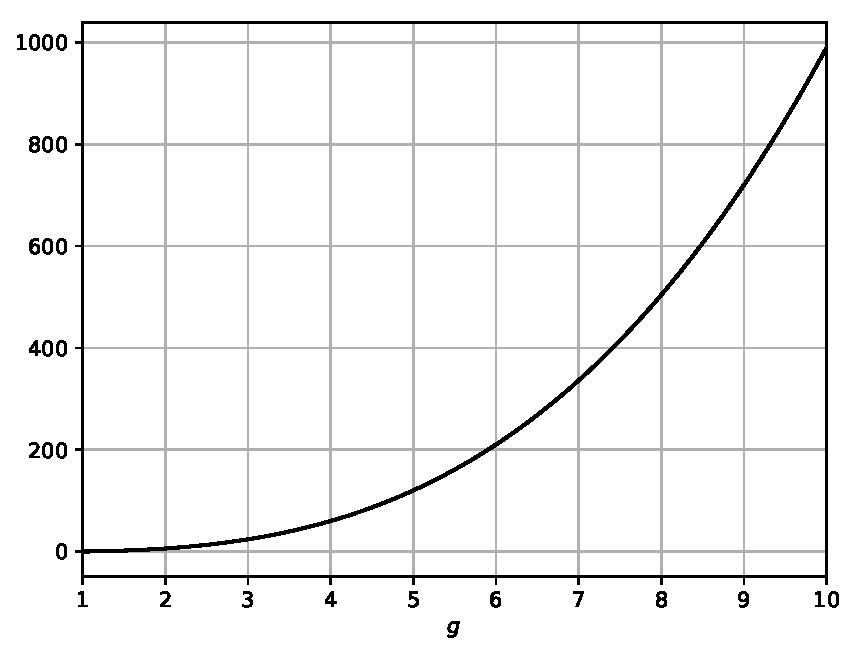
\includegraphics[width=7cm]{figs/ex_2_6_g}
    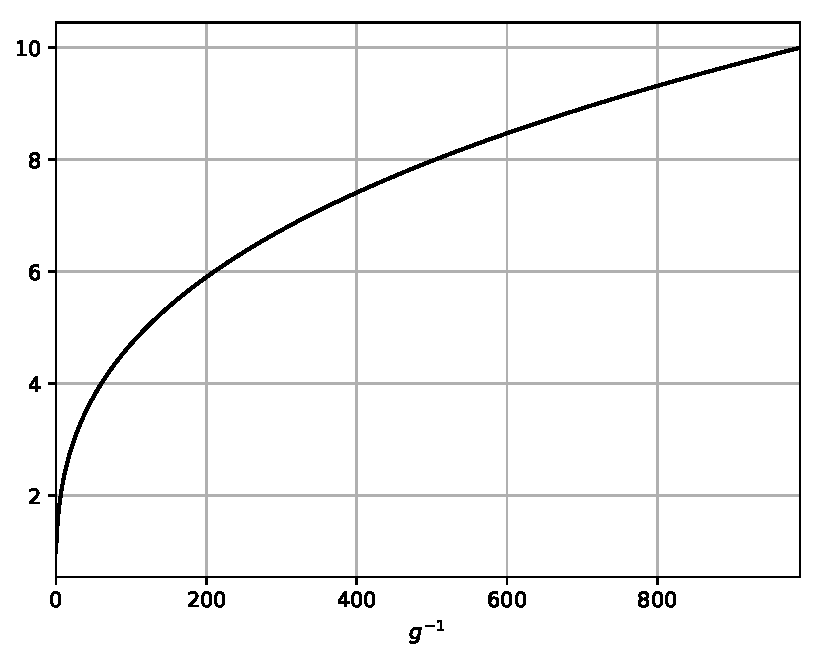
\includegraphics[width=7cm]{figs/ex_2_6_gi}
    % Need a blank line here for some dumb reason
    
  }
}
